\section{Introduction}
\label{sec:introduction}
In this lab we report we explore the effect of the second harmonic generation. Since it is derived
from non-linear optics, we will only give a short introduction in the theory and focus on the
observations.

In the second harmonic generation, also called ``frequency doubling``, two photons with the same
frequency interact in a
medium and ``merge`` into a new photon. The newly created photon has double the energy, or half the wavelength
compared to a photon of the initial state. A graphic showing the energy scheme is provided in
\autoref{fig:energy_scheme}.

There are requirements the material must fulfill: It must not have an inversion symmetry, since a
symetric potential would lead to resonance with fourier coefficients in uneven order only (i.e.
second order is vanishing). Therefore, surfaces and interface can be usefull.
\begin{figure}
    \centering
    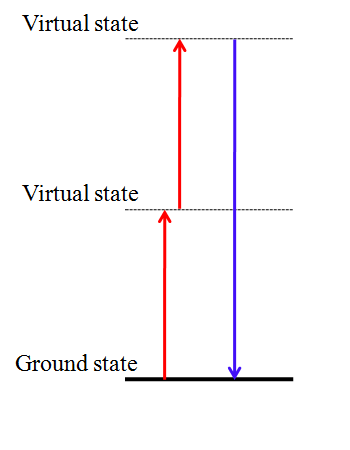
\includegraphics[width=0.3\textwidth]{media/Energy_level_scheme_of_SHG.png}
    \caption{Energy level scheme of SHG process. Taken from \cite{energy_level_scheme}.}
    \label{fig:energy_scheme}
\end{figure}

